\chapter{Análise exploratória do conjunto de dados}\label{anuxe1lise-exploratuxf3ria-do-conjunto-de-dados}
As contagens deste capítulo e dos experimentos subsequentes referem-se a três recortes com denominadores distintos: o universo cadastral histórico (69.895 UCs, das quais 65.762 constam como ligadas), o consolidado exploratório de quatro cortes usado no perfilamento inicial (66.099 UCs e 262.849 janelas) e as coortes de inferência fora do período de ajuste (65.686 UCs em 19/11/2026 e 65.640 em 25/11/2026).
\section{Caracterização cadastral, espacial e tecnológica}
O cadastro histórico reuniu 69.895 UCs, 72.707 registros de instalação e 72.661 NIOs distintos. Identificaram-se 1.288 UCs com mais de um medidor ao longo do histórico, 46 NIOs associados a múltiplas UCs e 1.480 registros de retirada. A diferença entre a contagem de linhas de instalação e a de UCs traduziu relações de substituição e reutilização. Na ausência de vigência, as mesmas relações poderiam transferir observações entre consumidores.

No recorte cadastral de instalações ligadas, encontraram-se 67.479 medidores em 65.762 UCs. Os inteligentes do grupo B representaram a maior parte do parque. Entre esses medidores, contaram-se 29.677 monofásicos, 25.466 bifásicos, 5.955 trifásicos e 3.083 classificados como monofásicos rurais. A Tabela \ref{parque} usa medidores ligados como denominador. A população analítica do corte OOT dependeu de outras condições de seleção.

\begin{table}[htbp]\centering\small\caption{Composição do parque de medição ligado}\label{parque}
\begin{tabular}{>{\raggedright\arraybackslash}p{\dimexpr 0.3333333333333333\linewidth-2\tabcolsep\relax}>{\raggedright\arraybackslash}p{\dimexpr 0.3333333333333333\linewidth-2\tabcolsep\relax}>{\raggedright\arraybackslash}p{\dimexpr 0.3333333333333333\linewidth-2\tabcolsep\relax}}\toprule
Tecnologia e grupo & Medidores & Fração do parque \\ \midrule
Inteligente, grupo B & 64.181 & 95,11\% \\
Inteligente, grupo A & 221 & 0,33\% \\
Convencional, grupo A & 1.617 & 2,40\% \\
Convencional, grupo B & 1.460 & 2,16\% \\
Total & 67.479 & 100,00\% \\
\bottomrule\end{tabular}
\par\small Fonte: elaboração própria a partir dos dados e métodos do estudo.
\end{table}
A hierarquia cadastral apresentou 23 alimentadores distintos. Na distribuição do consolidado de 66.099 UCs, a agregação produziu 18 circuitos identificados e uma categoria residual de 4.694 UCs sem alimentador. O maior circuito reuniu 8.810 UCs. A Figura \ref{cobertura} apresenta os circuitos identificados em ordem de porte e a distribuição de cobertura da mesma população. Entre os agrupamentos com pelo menos 20 UCs, um circuito com 1.541 unidades reuniu 290 sinalizações (18,82\%), enquanto outro com 20 unidades não apresentou sinalizações. A heterogeneidade de porte e o denominador de cada taxa condicionaram a leitura espacial.

\begin{figure}[htbp]\centering\caption{Cobertura por janela e distribuição de UCs entre os alimentadores identificados}\label{cobertura}
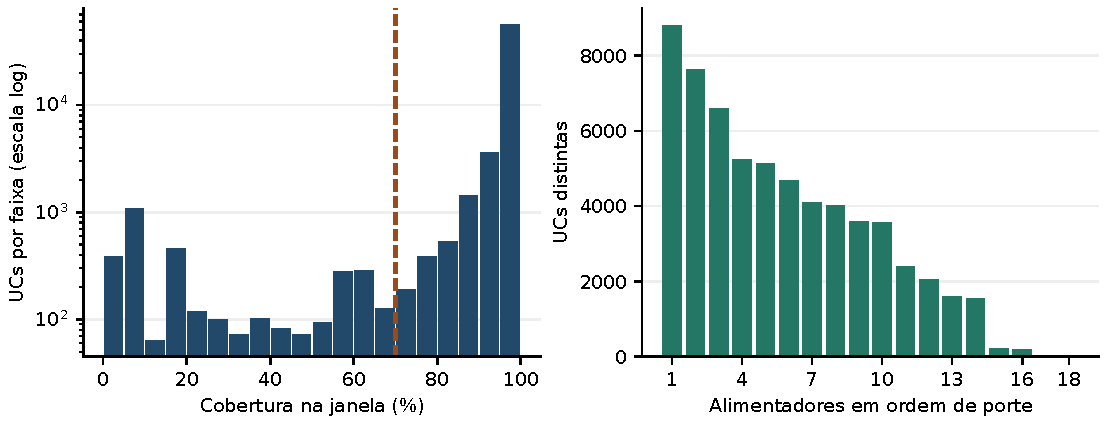
\includegraphics[width=0.96\textwidth,height=0.46\textheight,keepaspectratio]{figuras/cobertura.pdf}
\par\small Fonte: elaboração própria com base no consolidado exploratório.
\end{figure}
\section{Integridade temporal e seleção pela qualidade}
O inventário intervalar registrou 111 partições diárias entre 1\textordmasculine{} de agosto e 19 de novembro. Na camada de atributos por UC e dia, identificaram-se 102 datas entre 2 de agosto e 12 de novembro, intervalo com 103 dias civis. A data de 1\textordmasculine{} de outubro não constou do calendário dessa camada. O calendário mediu presença de partições. A completude individual foi avaliada separadamente, por janela.

Na última janela de cada UC do consolidado, a mediana de cobertura foi de aproximadamente 99,3\%. A faixa de 95\% a 100\% reuniu 56.570 UCs. Com limiar de 70\%, 62.766 UCs ficaram elegíveis e 3.333 permaneceram abaixo do filtro. Na Tabela \ref{selecao}, a diferença de energia mediana e de escore mostrou que a exclusão atingiu uma subpopulação com distribuição distinta. A menor energia estimada entre os inelegíveis também pode refletir a própria escassez de observações.

\begin{table}[htbp]\centering\small\caption{Comparação dos grupos de cobertura no consolidado de 66.099 UCs}\label{selecao}
\begin{tabular}{>{\raggedright\arraybackslash}p{\dimexpr 0.23\linewidth-2\tabcolsep\relax}>{\raggedright\arraybackslash}p{\dimexpr 0.14\linewidth-2\tabcolsep\relax}>{\raggedright\arraybackslash}p{\dimexpr 0.27\linewidth-2\tabcolsep\relax}>{\raggedright\arraybackslash}p{\dimexpr 0.16\linewidth-2\tabcolsep\relax}>{\raggedright\arraybackslash}p{\dimexpr 0.2\linewidth-2\tabcolsep\relax}}\toprule
Grupo & UCs & FA mediana (kWh/dia) & CV mediano & Escore mediano \\ \midrule
Cobertura \ensuremath{\geq} 70\% & 62.766 & 5,03 & 0,141 & 0,2321 \\
Cobertura \ensuremath{<} 70\% & 3.333 & 0,89 & 0,183 & 0,4245 \\
\bottomrule\end{tabular}
\par\small Fonte: elaboração própria a partir dos dados e métodos do estudo.
\end{table}
\section{Magnitude, forma e persistência}
A distribuição da mediana histórica de FA apresentou assimetria à direita. Os percentis 10, 50, 90 e 99 atingiram 0,314, 4,936, 11,068 e 55,060 kWh/dia, respectivamente. A média atingiu 7,001 kWh/dia. No diagrama de dispersão com 5.000 observações, valores de magnitude semelhante corresponderam a dispersões diferentes. A Figura \ref{dispersao} mostra também os perfis horários convertidos em frações da soma de suas 24 componentes para comparar forma.

\begin{figure}[htbp]\centering\caption{Dispersão robusta do consumo e formas horárias de carga da amostra exploratória}\label{dispersao}
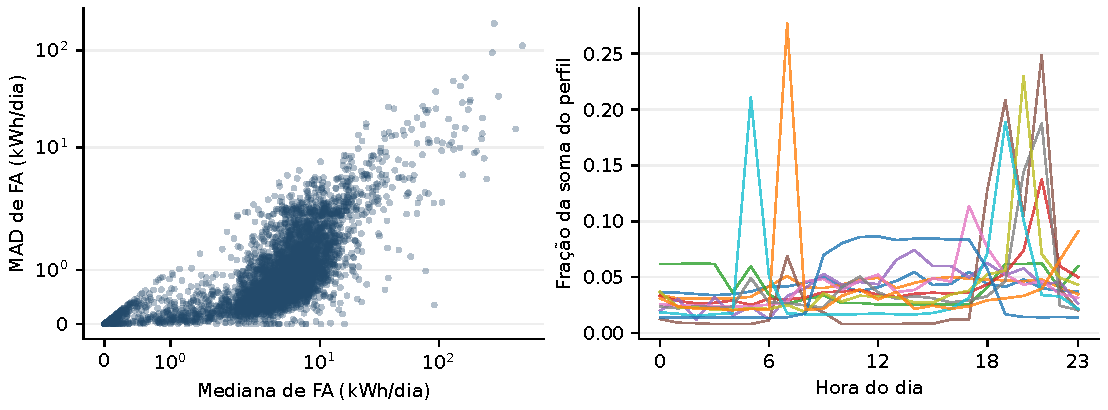
\includegraphics[width=0.96\textwidth,height=0.46\textheight,keepaspectratio]{figuras/dispersao.pdf}
\par\small Fonte: elaboração própria com base na amostra de atributos e nos perfis horários.
\end{figure}
Duas UCs exemplificaram essa diferença em 4 de novembro. Para 934***50 e 116****57, as medianas atingiram 20,382 e 19,224 kWh/dia, enquanto os MADs alcançaram 0,051 e 16,564 kWh/dia. Os fatores de carga foram 0,973 e 0,150, respectivamente. A cobertura de ambas foi 99,44\%. Na Figura \ref{perfil}, a primeira curva permaneceu próxima de 0,85 kWh por hora, e a segunda concentrou a energia entre a manhã e o início da tarde. A comparação de 168 horas registrou máximos de 0,933 e 7,03 kWh por hora. A escala diária aproximou os dois casos, mas a distribuição intradiária os distinguiu.

\begin{figure}[htbp]\centering\caption{Energia horária de duas UCs com medianas diárias próximas}\label{perfil}
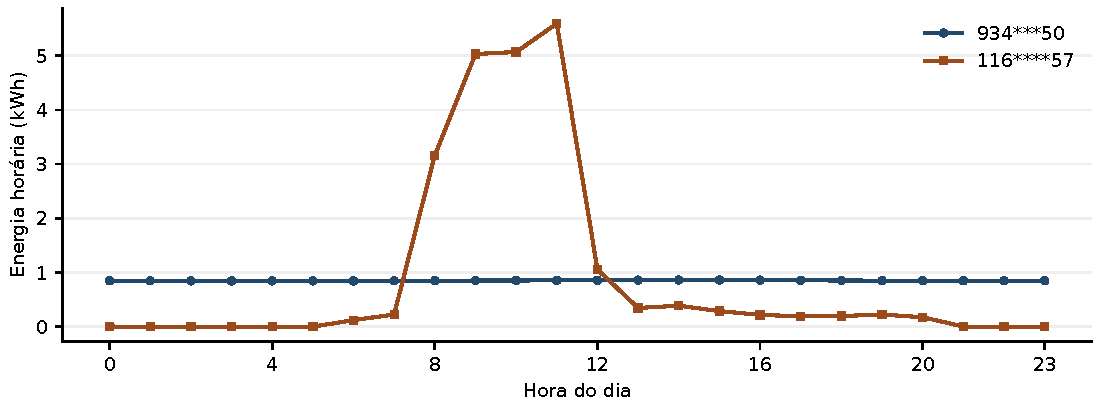
\includegraphics[width=0.96\textwidth,height=0.46\textheight,keepaspectratio]{figuras/perfil.pdf}
\par\small Fonte: elaboração própria com base nas medições intervalares do par de UCs.
\end{figure}
No painel operacional horário, a escala robusta parte de \(1{,}4826\,\mathrm{MAD}\), estimativa do desvio-padrão sob normalidade. O código aplica pisos relativos à mediana local e à escala global e um piso absoluto. A faixa horária se estende de três escalas abaixo da mediana, limitada inferiormente a zero, a 3,5 escalas acima. A Figura~\ref{semana} compara a dispersão diária com a maior energia observada em uma hora da semana. As medianas diárias próximas coexistem com uma diferença de mais de sete vezes entre os máximos horários.

\begin{figure}[htbp]\centering\caption{Dispersão diária e máximo horário observado em 168 horas}\label{semana}
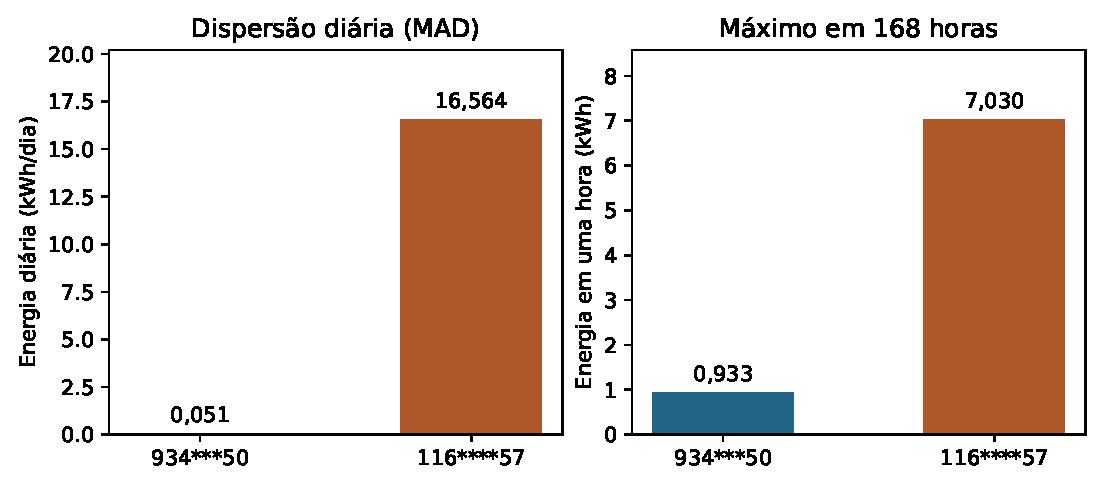
\includegraphics[width=.96\linewidth]{figuras/semana.pdf}
\par\small Fonte: elaboração própria a partir das estatísticas do par de UCs.
\end{figure}
A distribuição histórica de sequências consecutivas de dias sem consumo ou com perfil atípico apresentou 478 UCs com duração positiva, das quais 197 tiveram valor superior a 30 dias na variável agregada. A amplitude da variável ultrapassou a janela nominal de 30 dias e exigiu separar o contador histórico acumulado do indicador de proporção em janela fixa da Equação \eqref{dias}. Não se atribuiu a duração máxima dessa distribuição a nenhum dos casos longitudinais apresentados a seguir.
